%%
%% This is file `tikzposter-template.tex',
%% generated with the docstrip utility.
%%
%% The original source files were:
%%
%% tikzposter.dtx  (with options: `tikzposter-template.tex')
%% 
%% This is a generated file.
%% 
%% Copyright (C) 2013 by Pascal Richter and Richard Barnard
%% 
%% This file may be distributed and/or modified under the
%% conditions of the LaTeX Project Public License, either
%% version 2.0 of this license or (at your option) any later
%% version. The latest version of this license is in:
%% 
%% http://www.latex-project.org/lppl.txt
%% 
%% and version 2.0 or later is part of all distributions of
%% LaTeX version 2013/12/01 or later.
%% 


\documentclass{tikzposter} %Options for format can be included here

\usepackage{pgfplots}
\pgfplotsset{compat=newest}
\usepackage[utf8]{inputenc}
\usepackage{amsmath}
\usepackage{amsfonts}
\usepackage{amssymb}
\usepackage{wrapfig}
\usepackage{tikz}



% Title, Author, Institute
\title{Dykstra's projection algorithm in multiresolution analysis}
\author{Lutz Künneke, Jan Lebert}
\institute{CUDA Lab Course 2014, Institut für Numerische und Angewandte Mathematik}
%\titlegraphic{\includegraphics[height=0.08\textheight]{CUDA_Teaching_Center_3D.JPG}}


\iffalse
\makeatletter
\renewcommand\TP@maketitle{%
\centering
\begin{minipage}[b]{0.8\linewidth}
	\centering
	\color{titlefgcolor}
	{\bfseries \Huge \@title \par}
	\vspace*{1em}
	{\huge \@author \par}
	\vspace*{1em}
	{\LARGE \@institute}
\end{minipage}%
\iffalse
\tikz[remember picture,overlay]\node[scale=0.8,anchor=east,xshift=0.96\linewidth,yshift=4.5cm,inner sep=0pt] {%
\@titlegraphic
};
\tikz[remember picture,overlay]\node[scale=0.8,anchor=east,xshift=-0.6\linewidth,yshift=4.5cm,inner sep=0pt] {%
\@titlegraphic
};
\fi
}
\fi

% Choose Layout:  Default, Simple, Rays, Envelope, Wave, Desert, Sugar, Board
\usetheme{Rays}
%\usetitlestyle{Default}
%\usecolorstyle{Australia}
%\usecolorstyle[colorOne=black, colorTwo=red, colorThree=green, ]{Default}  % colorPalette=GrayBlue


\begin{document}
% Title block with title, author, logo, etc.
\maketitle[width=0.85\linewidth]

% Columns
\begin{columns}

	% FIRST column
	\column{0.50} % Width set relative to text width

	\block{Introduction}{
	In modern image analysis multiresolution methods have gained increasing interest in the last years.    
	Their application lies in the statistical inversion of
	\begin{align*}
		I = A*x + \epsilon
	\end{align*}
	where $A : \mathbb{R}^n \rightarrow \mathbb{R}^m$ is linear operator and $\epsilon$ is a vector represententing noise.

	A multiresolution estimator performs hypothesis tests on subsets of the estimated noise $\hat{\epsilon}$ in order to ensure normality on all scales. The resulting estimate is the underlying true signal of the noisy measurement in each subset with high probability.
	}
	\block{Implementation} {
	The hypothesis tests on subsets are calculated using Dykstra's Algorithm.
	Dykstra's Algorithm provides the projection on the intersection of convex sets $s \in \Omega$ given the projection $p_s$ on each set.
	Initialize $q_0^s = 0~\forall s \in \Omega$, then one iteration of Dykstra's Algorithm consists of $\forall s \in \Omega$
	\begin{align*} 
		x_{r+1} &= p_s \left( x_r - q_r^s \right) \\ 
		q_{r+1}^s &= x_{r+1} - x_r
	\end{align*}
	the algorithm is shown to converge towards the projection on the intersection of the $s \in \Omega$ given some $x_0$.\\
	The order in which the projections are performed is crucial for the convergence of the algorithm, therefore only non-overlapping 
	subsequent projections can be calculated in parallel. Due to this restriction we've developed an approximative version which uses
	subsets which are suitable for parallel computation with CUDA. \\
	The performance of the exact method is limited by the transfer rate of the PCIe bus.
	\begin{tikzfigure}[subset selection of exact {\bf (left)} and approximative {\bf (right)} method]
		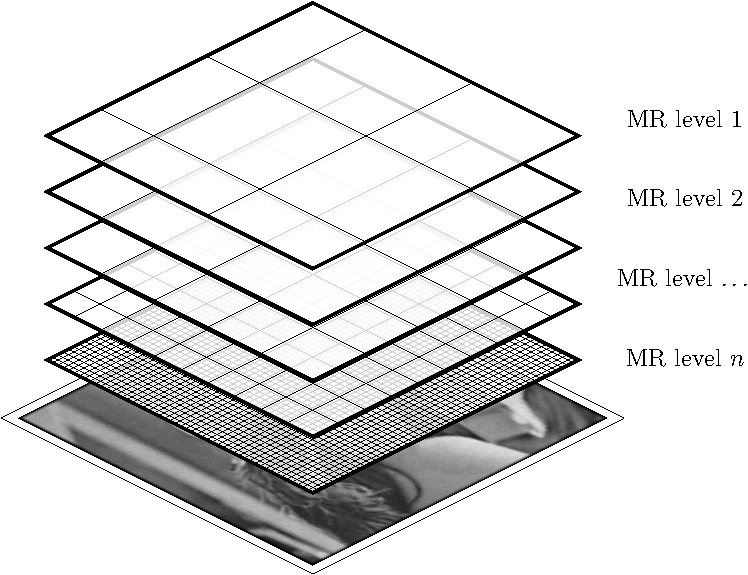
\includegraphics[width=0.22\textwidth]{dykstra_crop.pdf}
		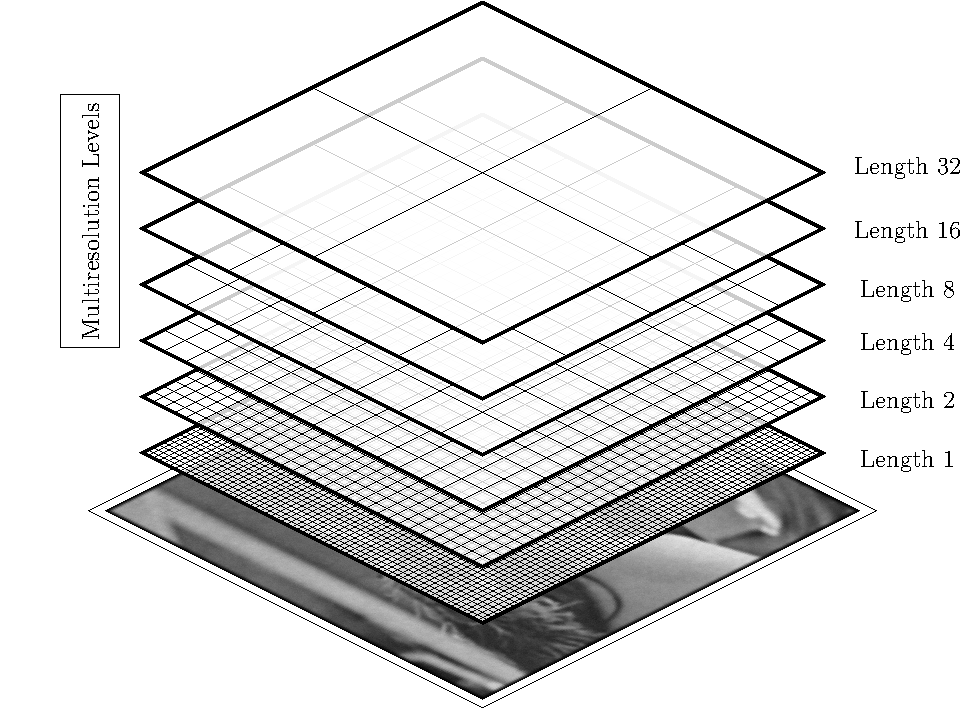
\includegraphics[width=0.22\textwidth]{dykstra_approx_crop.pdf}
	\end{tikzfigure}
	}

	\block{SOFI}{
	\begin{center}
		\begin{tikzfigure}[SOFI result without {\bf (left)} and with {\bf (right)} prior deconvolution]
			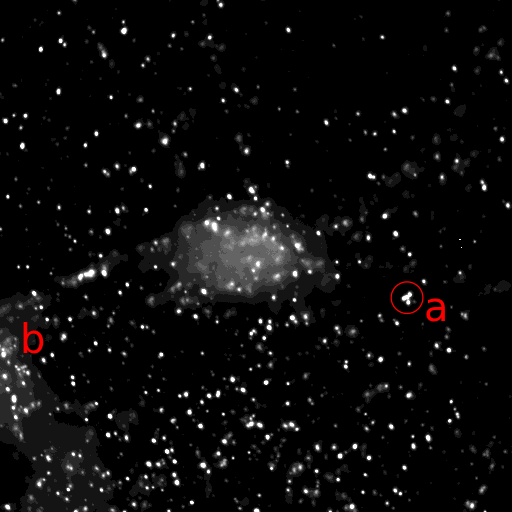
\includegraphics[width=0.22\textwidth]{/home/jan.lebert/Praktikum_2014/testsite/step-35/doc/images/sofi_result_analysis_orig.png}
			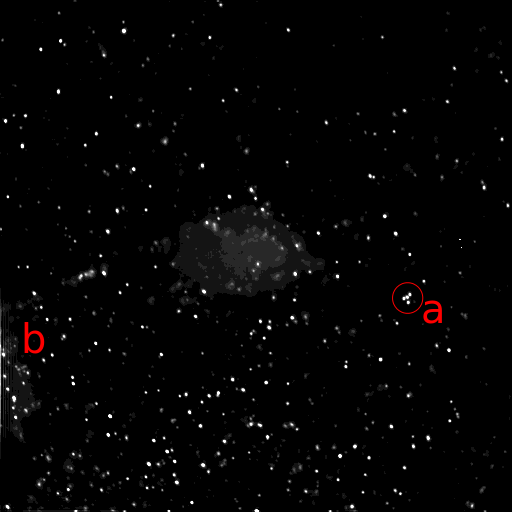
\includegraphics[width=0.22\textwidth]{/home/jan.lebert/Praktikum_2014/testsite/step-35/doc/images/sofi_result_analysis.png}
		\end{tikzfigure}
	\end{center}

	\begin{tabular}{l l}
		\begin{minipage}{0.24\textwidth}
			In order to apply the SOFI algorithm \cite{Dertinger-poster} blinking nanobeads are attached to some structure of interest.
			The nanobeads show uncorrelated blinking. By calculating the spatial and temporal
			correlation between pixels one can improve the overall resolution. \\ 
			We analysed a movie with 3500 frames and a duration of 10ms per frame using the approximative method.
			To produce the right hand image we applied a statistical multiresolution estimator on each image before application
			of SOFI. The resulting image shows smaller point spread functions {\bf (a)}, but our algorithm introduces
			some artefacts at the boundaries {\bf (b)}.
		\end{minipage}\hspace{-0.9cm}
		&
		\begin{minipage}{0.22\textwidth}
			%\resizebox {0.25\textwidth} {0.25\textwidth} {
			\begin{center}

				\begin{tikzpicture}
					\begin{semilogyaxis}[
						title={power spectral density},
						xlabel={$\left|k\right|^2$},
						ylabel={psd},
						grid=major,
						legend entries={SOFI result, SOFI w. prior deconvolution},
						width=0.8\textwidth,
						legend cell align=left,
						x tick label style={font=\tiny},
						x label style={font=\small},
						y tick label style={font=\tiny},
						y label style={font=\small},
						legend style={font=\small},
						title style={font=\small}
						]
						\addplot+[mark=*, dotted] table[x=dof,y=SOFI] {/home/jan.lebert/Praktikum_2014/testsite/step-35/doc/images/psd_data};
						\addplot+[mark=*, dotted] table[x=dof,y=DSOFI] {/home/jan.lebert/Praktikum_2014/testsite/step-35/doc/images/psd_data};
					\end{semilogyaxis}
				\end{tikzpicture}
			\end{center}
			%}
			\end{minipage}
		\end{tabular}
		The power spectral density {\bf (right)} indicates a favourable resolution in our result.
		}

		%\note{Note with default behavior}
		\note[targetoffsetx=5cm, targetoffsety=20.5cm, angle=20, rotate=20]{real data}

		% SECOND column
		\column{0.50} % Second column with first block's top edge aligned with with previous column's top.

		\block{Lena}{
		The Dykstra Algorithm was applied within the estimator
		\begin{align*}
			\hat{x} = \text{argmin}_{x,e} G \left( e \right) + R \left( x \right) \text{ s.t. } I = A*x + e 
		\end{align*}
		with noise $e \sim N \left( 0 , \sigma^2 \right)$, blur $A: \mathbb{R}^n \rightarrow \mathbb{R}^m$ and signal $x$.
		$R$ is a regularization and $G$ the characteristic function of the multiresolution.
		\begin{center}
			\begin{tikzfigure}[original image {\bf (left)}, test image with simulated blur and gaussian noise {\bf (right)}]
				\label{fig:fig2}
				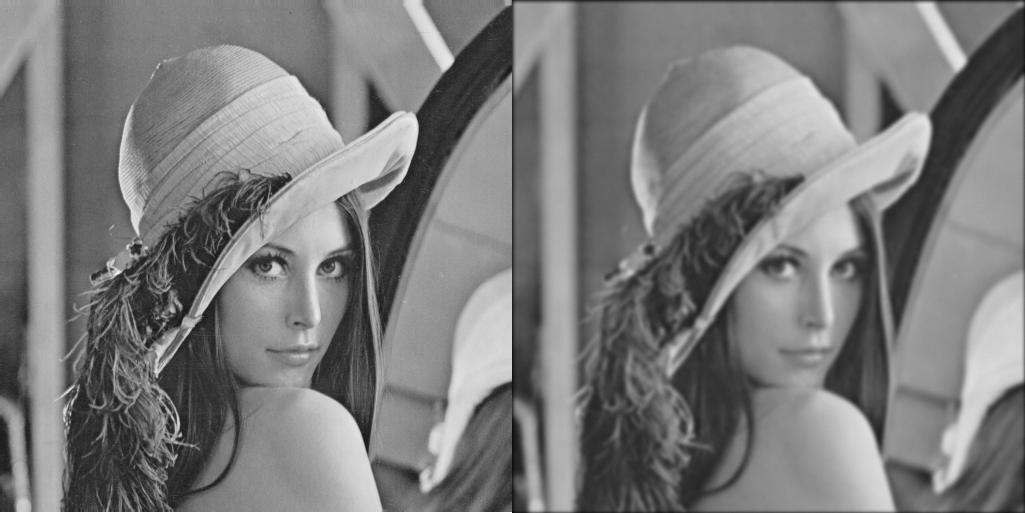
\includegraphics[width=0.366\textwidth]{/home/jan.lebert/Praktikum_2014/testsite/step-35/doc/images/lena_noise.png}
			\end{tikzfigure}
			\begin{tikzfigure}[Statistical Multiresolution Estimate using exact Dykstra {\bf (left)} and approximative Dykstra {\bf (right)}]
				\label{fig:fig2}
				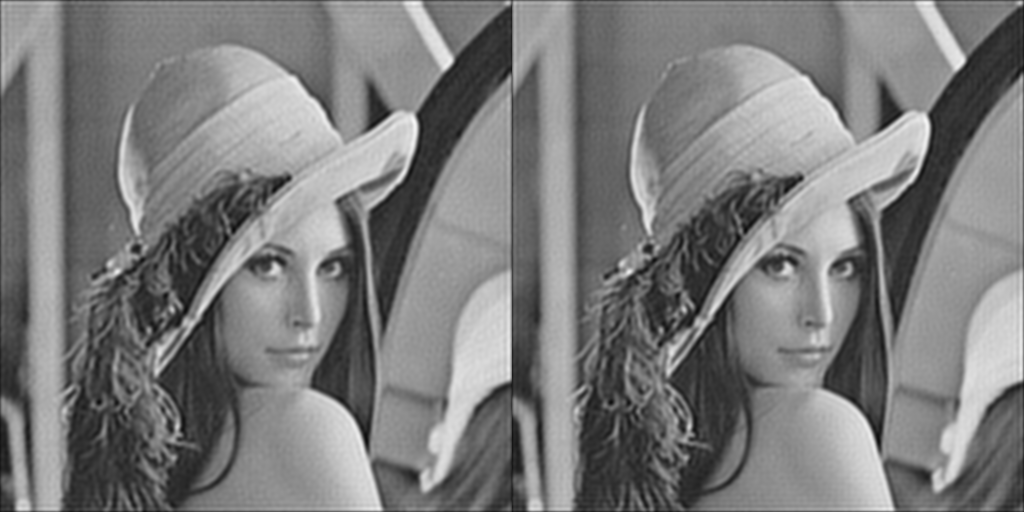
\includegraphics[width=0.366\textwidth]{/home/jan.lebert/Praktikum_2014/testsite/step-35/doc/images/lena_results.png}
			\end{tikzfigure}
		\end{center}

		The images show results of the estimator on simulated data. The estimator reduces the blur and noise to a certain extent.
		There is no visible difference between exact and approximative projection algorithm. 
		}
		\note[targetoffsetx=5cm, targetoffsety=25.8cm, rotate=20]{simulated data}

		\block{Speedup} {
		\begin{tabular}{l l}
			\begin{minipage}[t]{0.24\textwidth}
				\begin{center}\hspace{-3.5cm}
					\begin{tikzpicture}
						\begin{loglogaxis}[
							title={Runtime},
							xlabel={Edge length of quadratic image [px]},
							ylabel={Runtime [s]},
							grid=major,
							legend entries={GPU exact, GPU approx, CPU},
							legend pos=north west,
							legend cell align=left,
							label style={font=\small},
							x tick label style={font=\tiny},
							x label style={font=\small},
							y tick label style={font=\tiny},
							y label style={font=\small},
							legend style={font=\small},
							title style={font=\small},
							width=0.8\textwidth,
							xmax=3072
							]
							\addplot table {/home/jan.lebert/Praktikum_2014/testsite/step-35/doc/images/speed_log.exact.plot};
							\addplot table {/home/jan.lebert/Praktikum_2014/testsite/step-35/doc/images/speed_log.approx.plot};
							\addplot table {/home/jan.lebert/Praktikum_2014/testsite/step-35/doc/images/speed_log.cpu.plot};
						\end{loglogaxis}
					\end{tikzpicture}
				\end{center}
			\end{minipage}\hspace{-3.5cm}
			&
			\begin{minipage}[t]{0.24\textwidth}
				\begin{center}
					\begin{tikzpicture}
						\begin{loglogaxis}[
							title={Speedup },
							xlabel={Edge length of quadratic image [px]},
							ylabel={Speedup = $\frac{T_{\text{gpu}}}{T_{\text{cpu}}}$},
							grid=major,
							legend entries={GPU exact, GPU approx},
							legend pos=north west,
							legend cell align=left,
							label style={font=\small},
							x tick label style={font=\tiny},
							x label style={font=\small},
							y tick label style={font=\tiny},
							y label style={font=\small},
							legend style={font=\small},
							title style={font=\small},
							width=0.8\textwidth,
							xmax=3072
							]
							\addplot table[x=px,y=exact] {/home/jan.lebert/Praktikum_2014/testsite/step-35/doc/images/speedup.data.plot};
							\addplot table[x=px,y=approx] {/home/jan.lebert/Praktikum_2014/testsite/step-35/doc/images/speedup.data.plot};
						\end{loglogaxis}
					\end{tikzpicture}
				\end{center}
			\end{minipage}
		\end{tabular}

		The left image compares runtime for three implementations of the projection algorithm, the right images shows the
		speedup of the CUDA implementations compared to the OpenMP parallelized CPU implementation. \\
		Notice that the approximative Dykstra uses a different algorithm than the CPU implementation, the exact method achieves a
		speedup of about 100.
		}

		% Second column - third block
		\block{References}{
		\renewcommand{\refname}{\vspace{-2em}}
		\bibliographystyle{plain}
		\bibliography{/home/jan.lebert/Praktikum_2014/testsite/step-35/doc/step-35.bib}
		\nocite{dykstra}
		}

		% Second column - A collection of blocks in subcolumn environment.

		% Bottomblock
		\block{}{
		\begin{wrapfigure}{r}{0.05\textwidth}\vspace{-1.0em}\hfill
			\includegraphics[width=0.043\textwidth]{CUDA_Teaching_Center_3D.JPG}
		\end{wrapfigure}
		This work was supported by the NVIDIA Teaching Center \mbox{Göttingen}, the source code is available as part of SciPAL as \emph{step-35}. 
		We thank Johannes Hagemann and Stephan Kramer for their help.
		}


	\end{columns}
	\end{document}



\endinput
%%
%% End of file `tikzposter-template.tex'.
